\chapter{多节点采集与统一事件化}

\section{节点近端持续采集}
\texttt{log-collector} 以节点近端部署方式持续读取日志新增内容。它不尝试在采集阶段完成复杂语义判断，而是尽快把一行原始日志转换为带来源、设备和时间信息的事件并写入原始事件流。这样可以把“日志产生速度”与“后续推理复杂度”解耦：采集器保持轻量，推理层则可以独立扩展实例或更换模型。

采集靠近数据源还有两项直接价值。第一，边缘快速路径不需要等待跨网传输；第二，原始日志可以优先留在边缘域，只有被路由选中的事件及裁剪后的上下文才进入云端。当前采集器按非空日志行事件化，时间窗口聚合、日志轮转与 inode 切换属于进一步增强项。

\section{多类节点的统一登记与接入状态}

在多节点采集开始前，管理端以统一设备记录维护节点标识、设备名称和就绪状态，使后续事件能够关联到稳定来源，而不依赖日志正文临时推断设备身份。Apache、Linux、Hadoop 和 ZooKeeper 等不同类型的日志源使用同一登记接口进入系统；采集适配可以因来源而变化，但节点状态查询、事件标识和后续处理契约保持一致。

\begin{figure}[htbp]
  \centering
  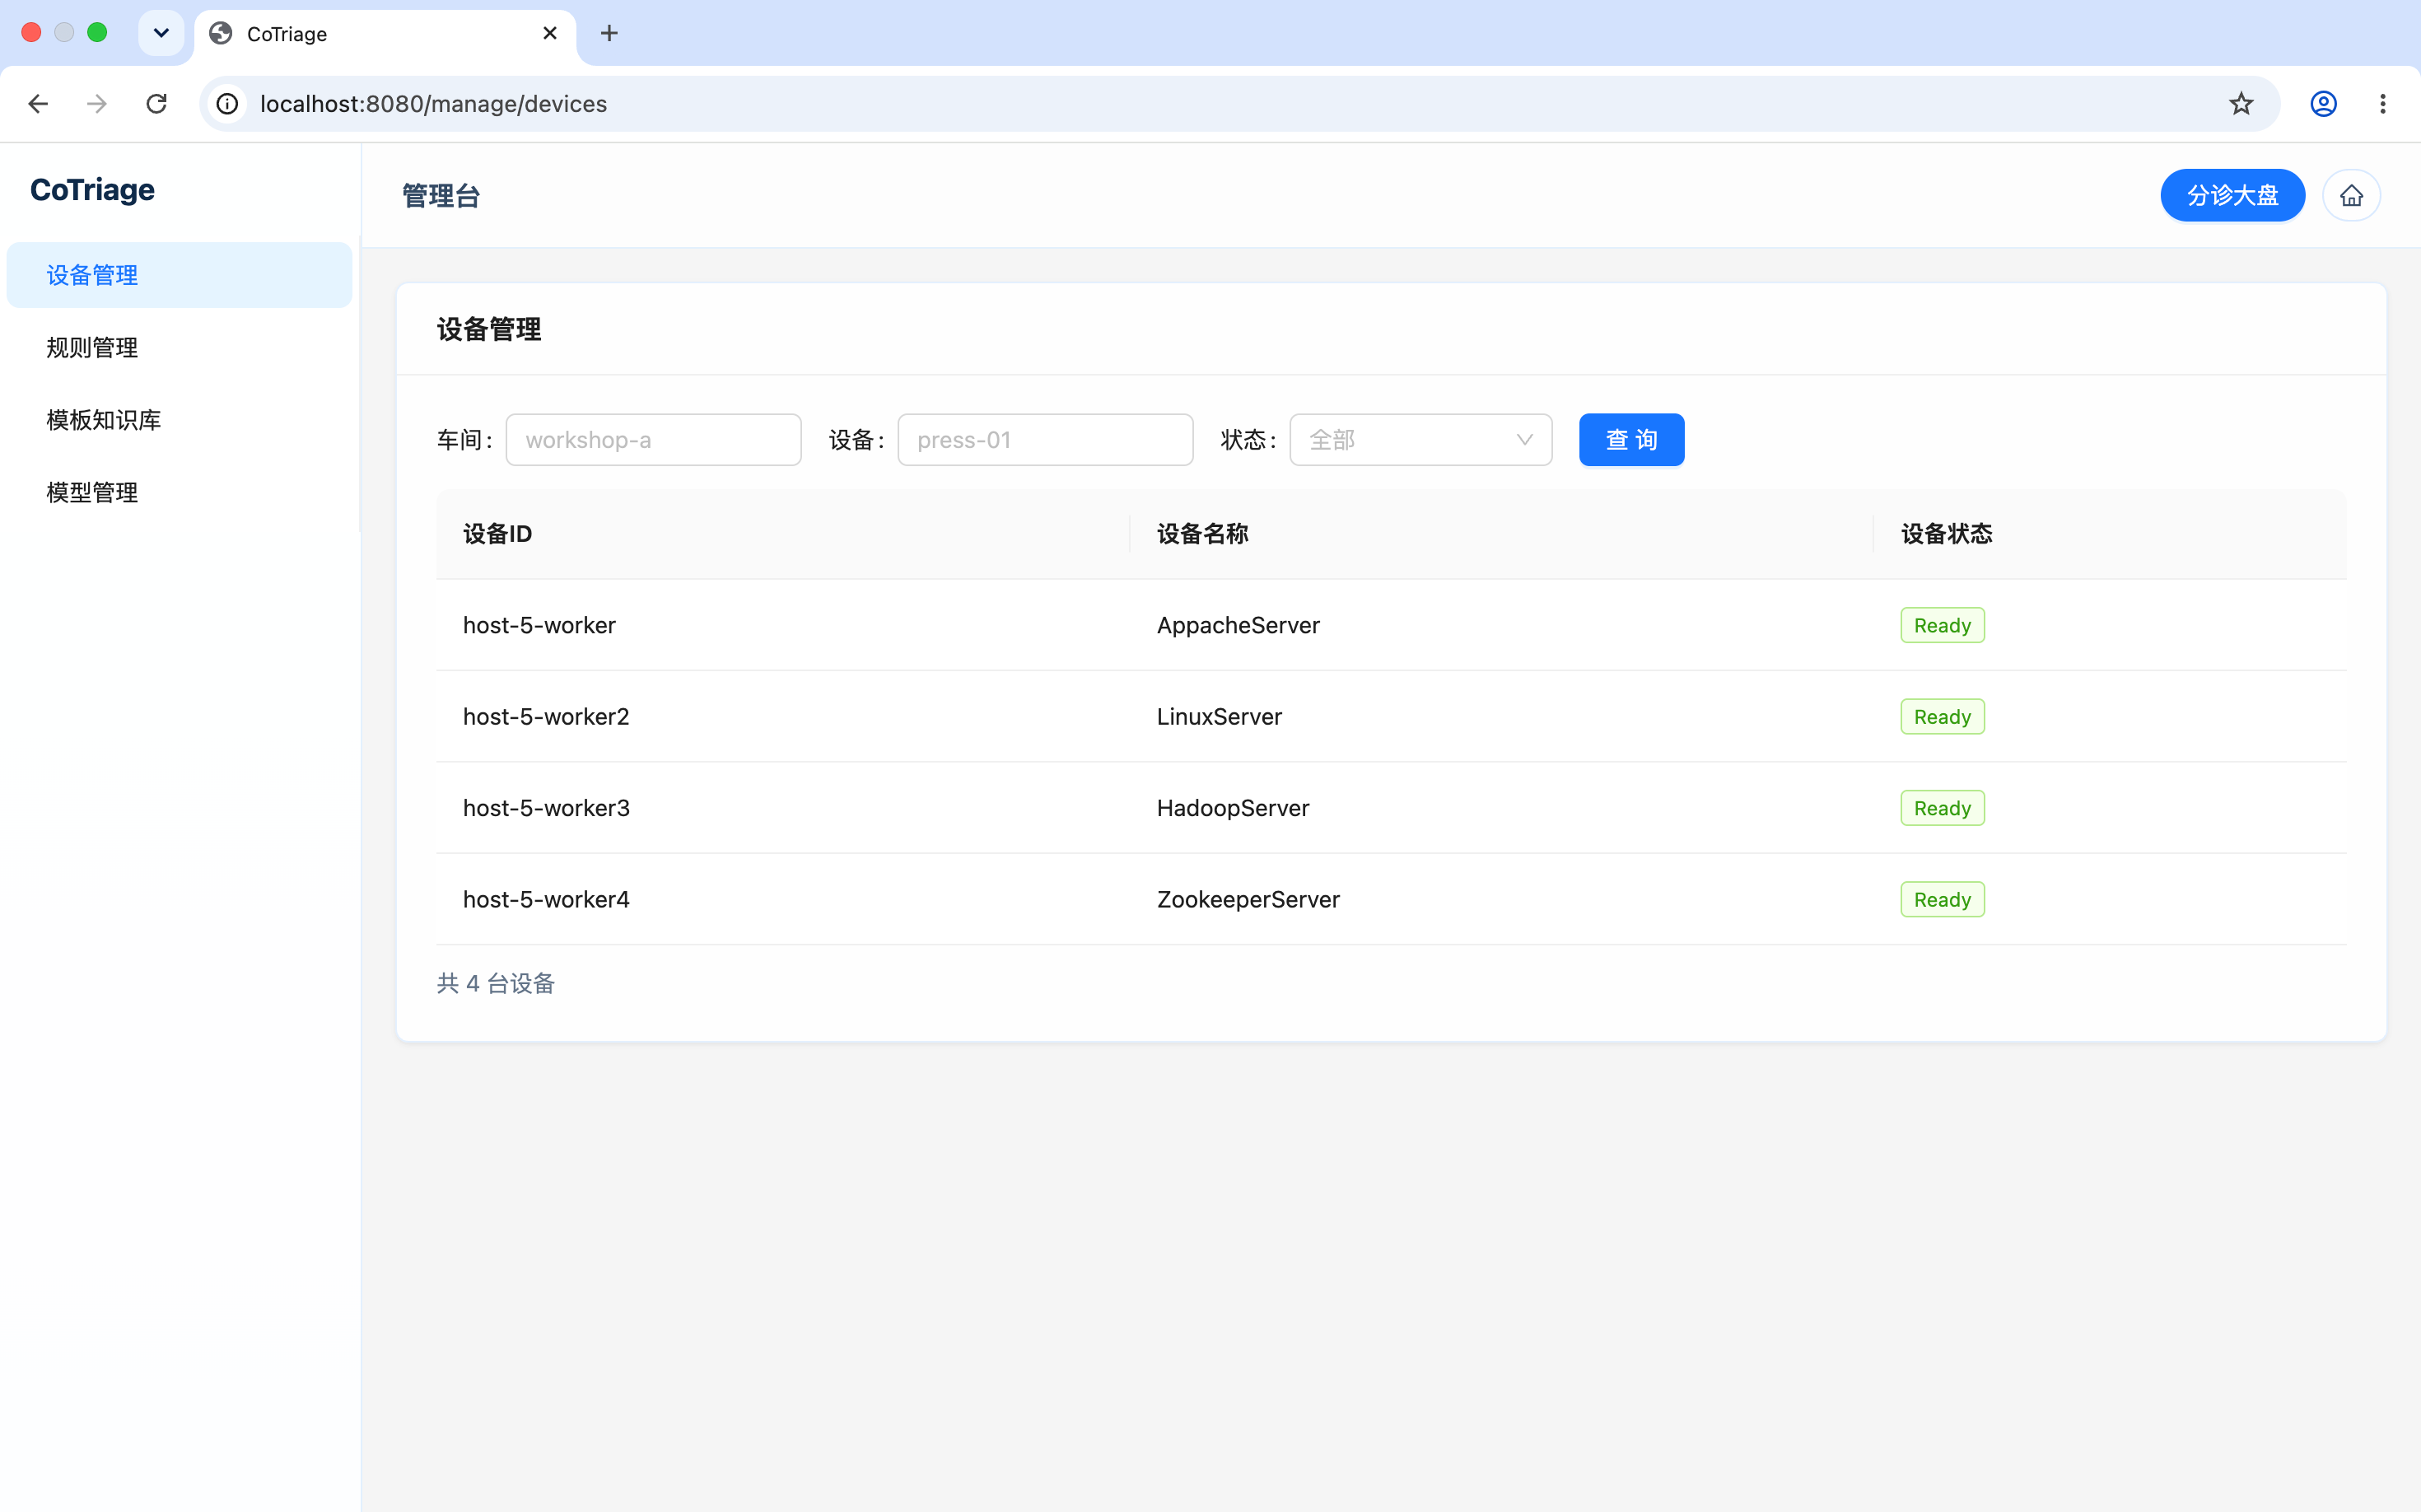
\includegraphics[width=0.90\textwidth]{figures/s-02-device-management.png}
  \caption{多类日志节点在管理端统一登记并呈现就绪状态}
  \label{fig:device-management}
\end{figure}

\cref{fig:device-management}展示了当前运行环境中的多类节点登记结果。该页面一方面验证采集链能够区分不同设备与日志来源，另一方面为事件流中的设备筛选、跨节点上下文聚合和运行状态下钻提供入口。图中数量仅反映截图时的登记情况，不用于推断系统扩展上限；节点规模变化主要由采集实例、Stream 消费组和后续处理服务的独立扩容承接。

\section{统一事件模型}
统一事件不是修改原始日志含义，而是在原文之外增加可跨组件复用的公共字段。核心字段分为四组。

\begin{table}[htbp]
  \centering
  \small
  \caption{统一事件的字段分组及其作用}
  \label{tab:event-fields}
  \begin{tabularx}{\textwidth}{>{\bfseries}p{0.17\textwidth} p{0.29\textwidth} X}
    \toprule
    字段组 & 代表字段 & 作用 \\
    \midrule
    身份与来源 & \texttt{event\_id}、设备、来源、时间 & 跨节点区分事件并支持时间排序 \\
    原始内容 & 原始日志、归一化模板、上下文摘要 & 保留诊断信息并支持模板复用 \\
    推理结果 & 类别、严重度、置信度、不确定性、路径、版本、时延 & 说明边缘如何形成当前判断 \\
    路由与状态 & 动作、分数、阈值、原因、预算、网络、队列快照 & 说明为何选择本地、云端或延期 \\
    \bottomrule
  \end{tabularx}
\end{table}

稳定的事件契约使规则引擎、模型服务和 Web 页面可以独立演进。即使某次判断更换了模型，\texttt{event\_id} 与版本字段仍能把该事件的原文、推理、路由和云端结果串联起来。

\section{实时事件流与推理路径}
\begin{figure}[htbp]
  \centering
  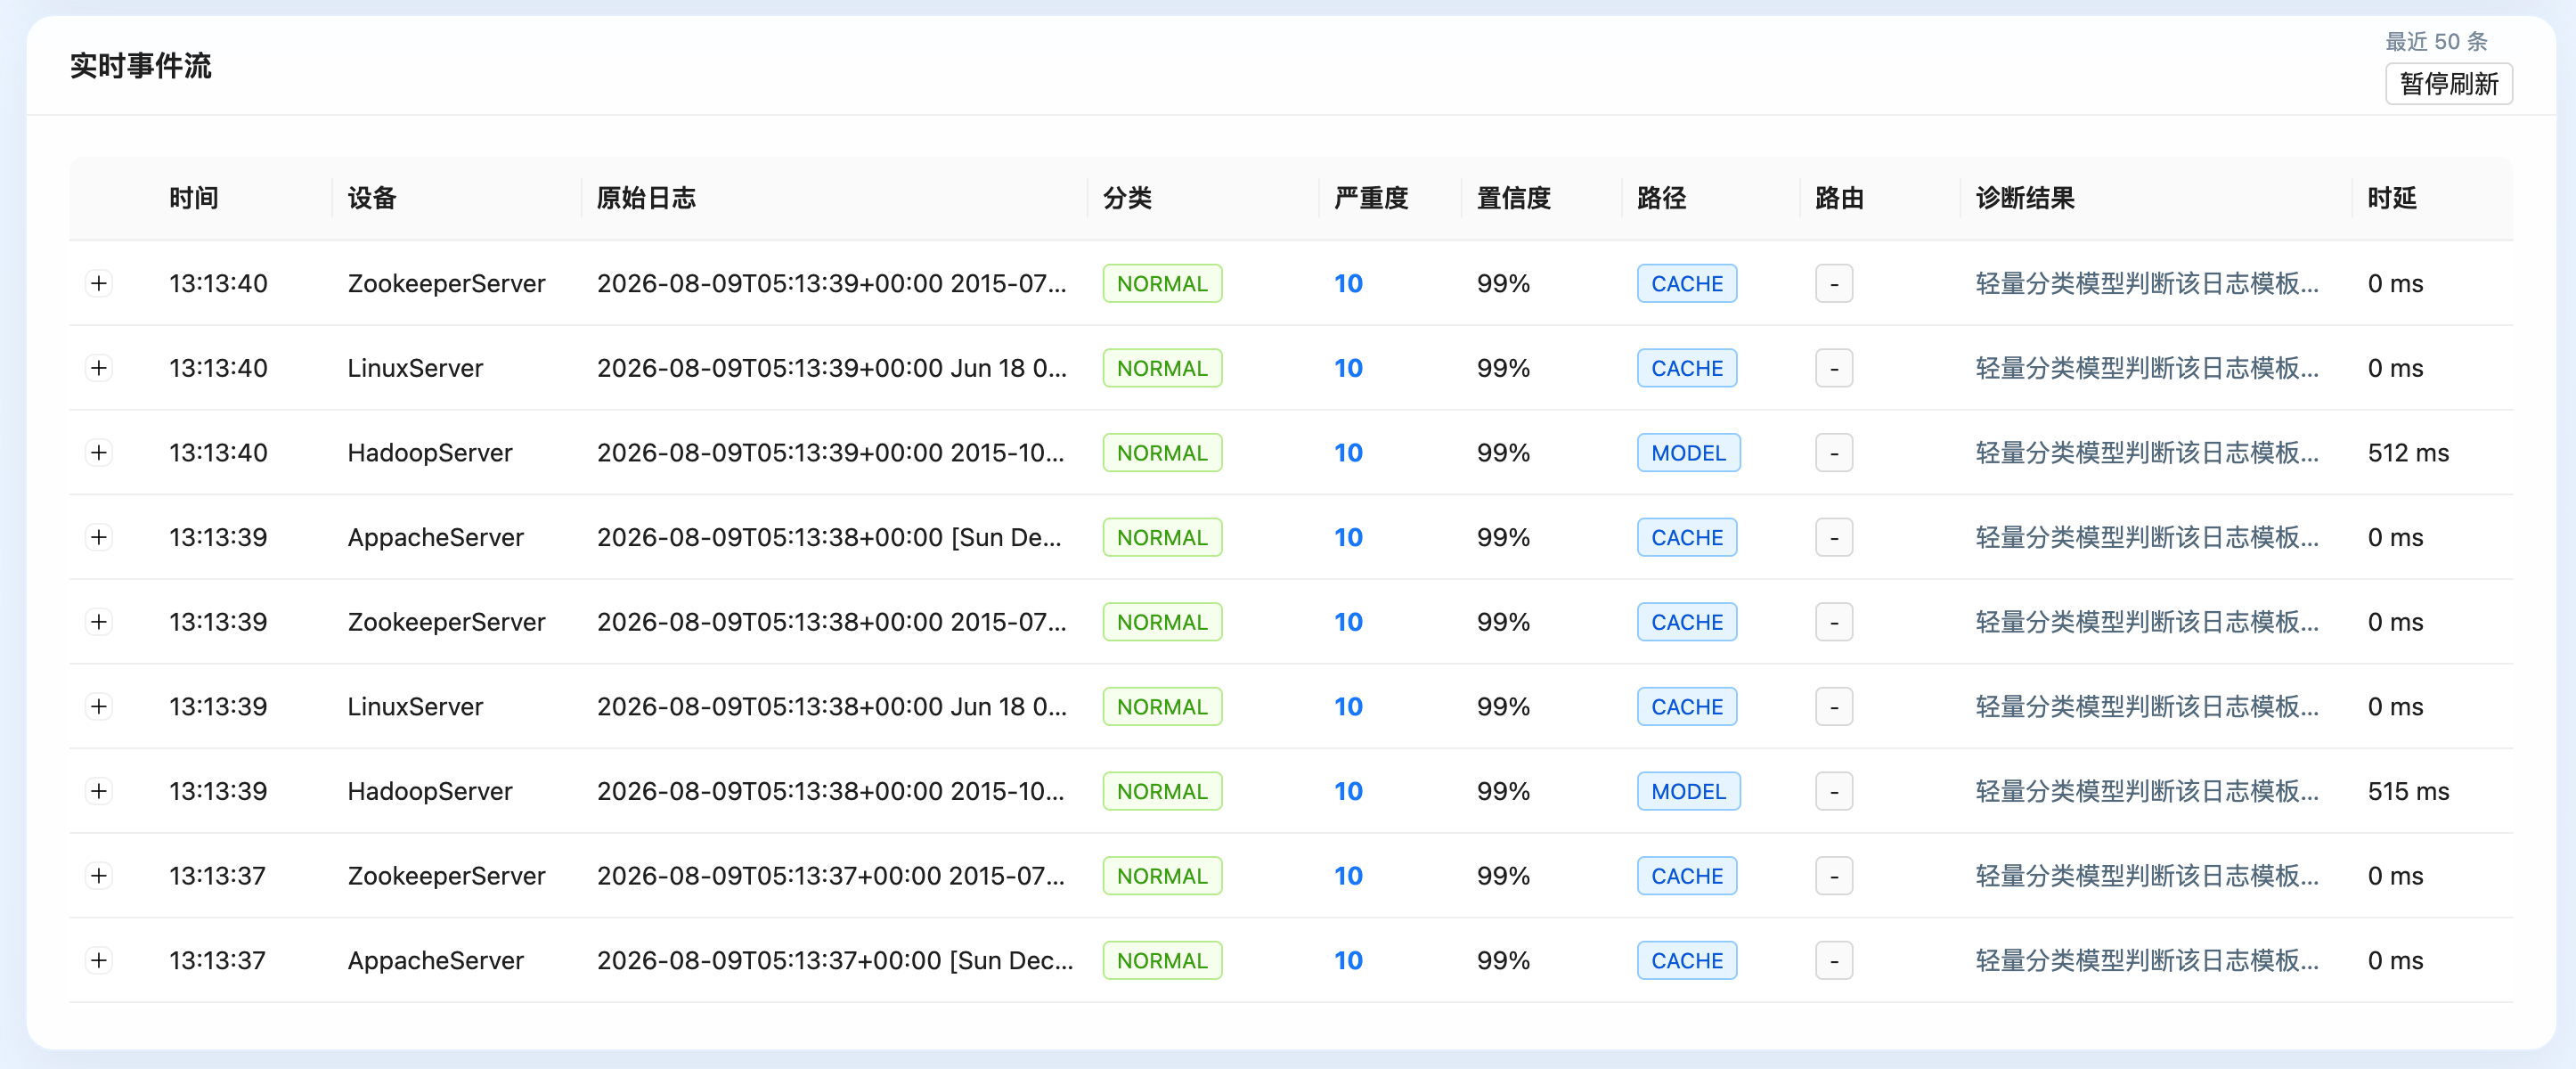
\includegraphics[width=0.98\textwidth]{figures/s-02d-realtime-event-stream-cache-model.png}
  \caption{统一事件流同时呈现不同设备与边缘推理路径}
  \label{fig:event-stream-cache-model}
\end{figure}

\cref{fig:event-stream-cache-model}在同一页面中展示了多个设备的原始日志、类别、严重度、置信度、推理路径、路由字段、诊断摘要和单事件耗时。画面中的 \texttt{CACHE} 与 \texttt{MODEL} 表明事件可以在不同边缘层级结束；表内耗时是各事件当次处理记录，不应直接替代运行窗口的平均值或 P95 指标。

\section{消息确认、幂等与追踪}
原始事件、推理结果、路由结果和云端请求分别进入独立 Stream。Consumer Group 让多个实例分担消费，ACK 表示消息已经完成当前阶段；已投递但未确认的消息进入 Pending Entries List。边缘推理已具备 Pending 接管机制，路由与云端网关仍需进一步统一接管策略。

系统将延迟确认和幂等组合使用：先完成持久化与下游发布，再确认当前消息；重试时依据幂等键复用既有状态，避免重复产生高成本调用。推理路径、模型版本、规则版本、时延和路由快照则进入观测面，使运维人员能够从驾驶舱下钻到单事件处理过程。

\section{从日志行到可操作事件}
一次完整处理可以概括为五步：采集器读取日志并生成唯一标识；边缘推理补充类别、风险与路径；RAISE 结合系统状态产生动作和解释；被选中的事件进入云端上下文聚合；最终结果通过数据库、消息流和 Web 页面被保存和展示。统一事件是这五步之间的公共语言，也是后续场景扩展和问题复盘的最小单位。
